\section{figures}

\begin{figure}[h]
\centering 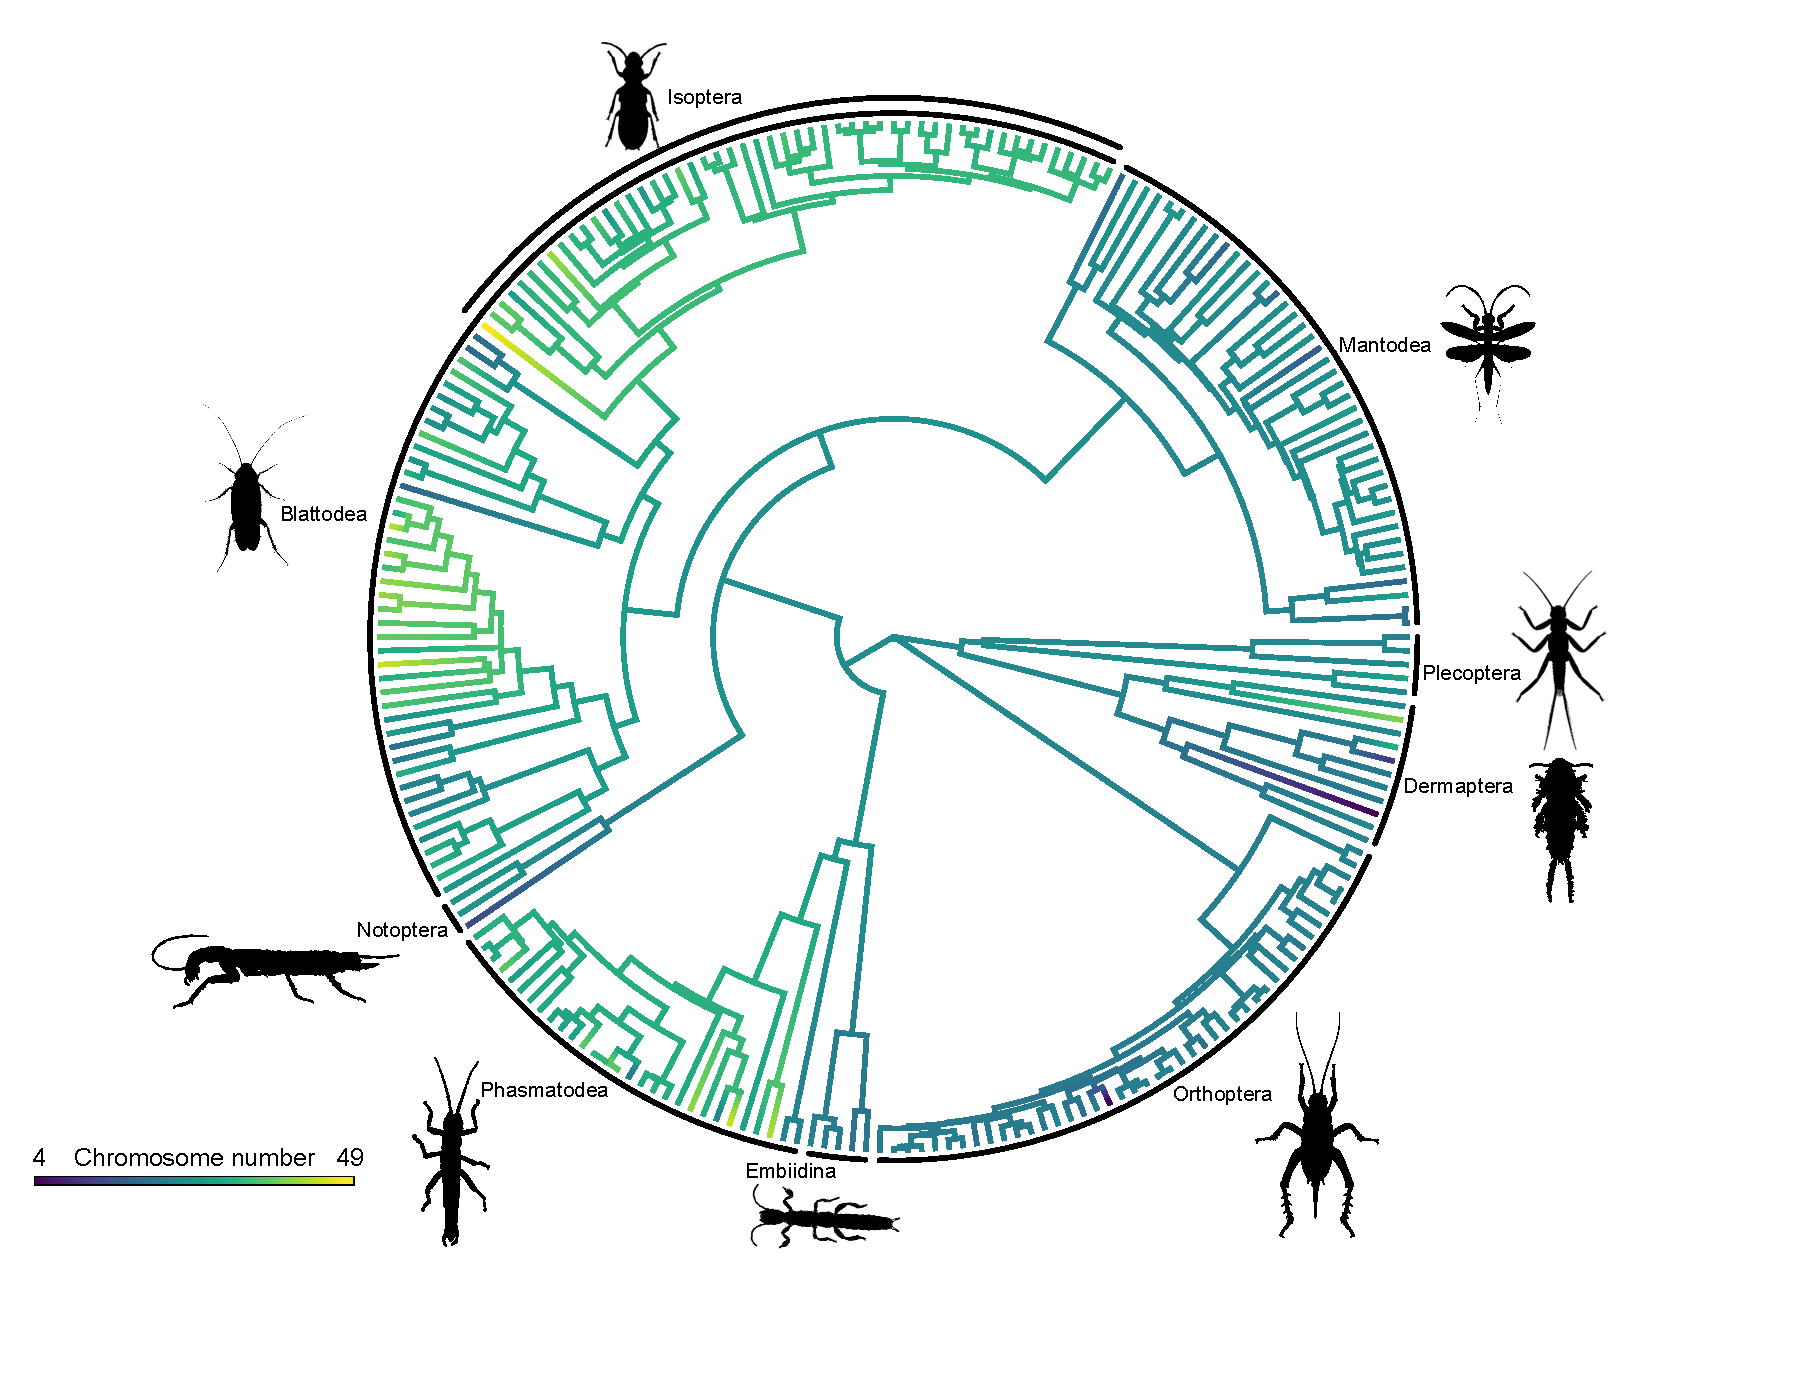
\includegraphics[width=1\textwidth]{figures/phylogenetic_tree.pdf}
\caption{One of the 100 trees from the posterior distribution with taxonomy and chromosome number displayed. The solid black line indicates the tips included in each order. Branches are coloured according to ancestral state estimates under a Brownian motion model. 
}
\label{fig:phyloplot}
\end{figure}

\begin{figure}
\centering 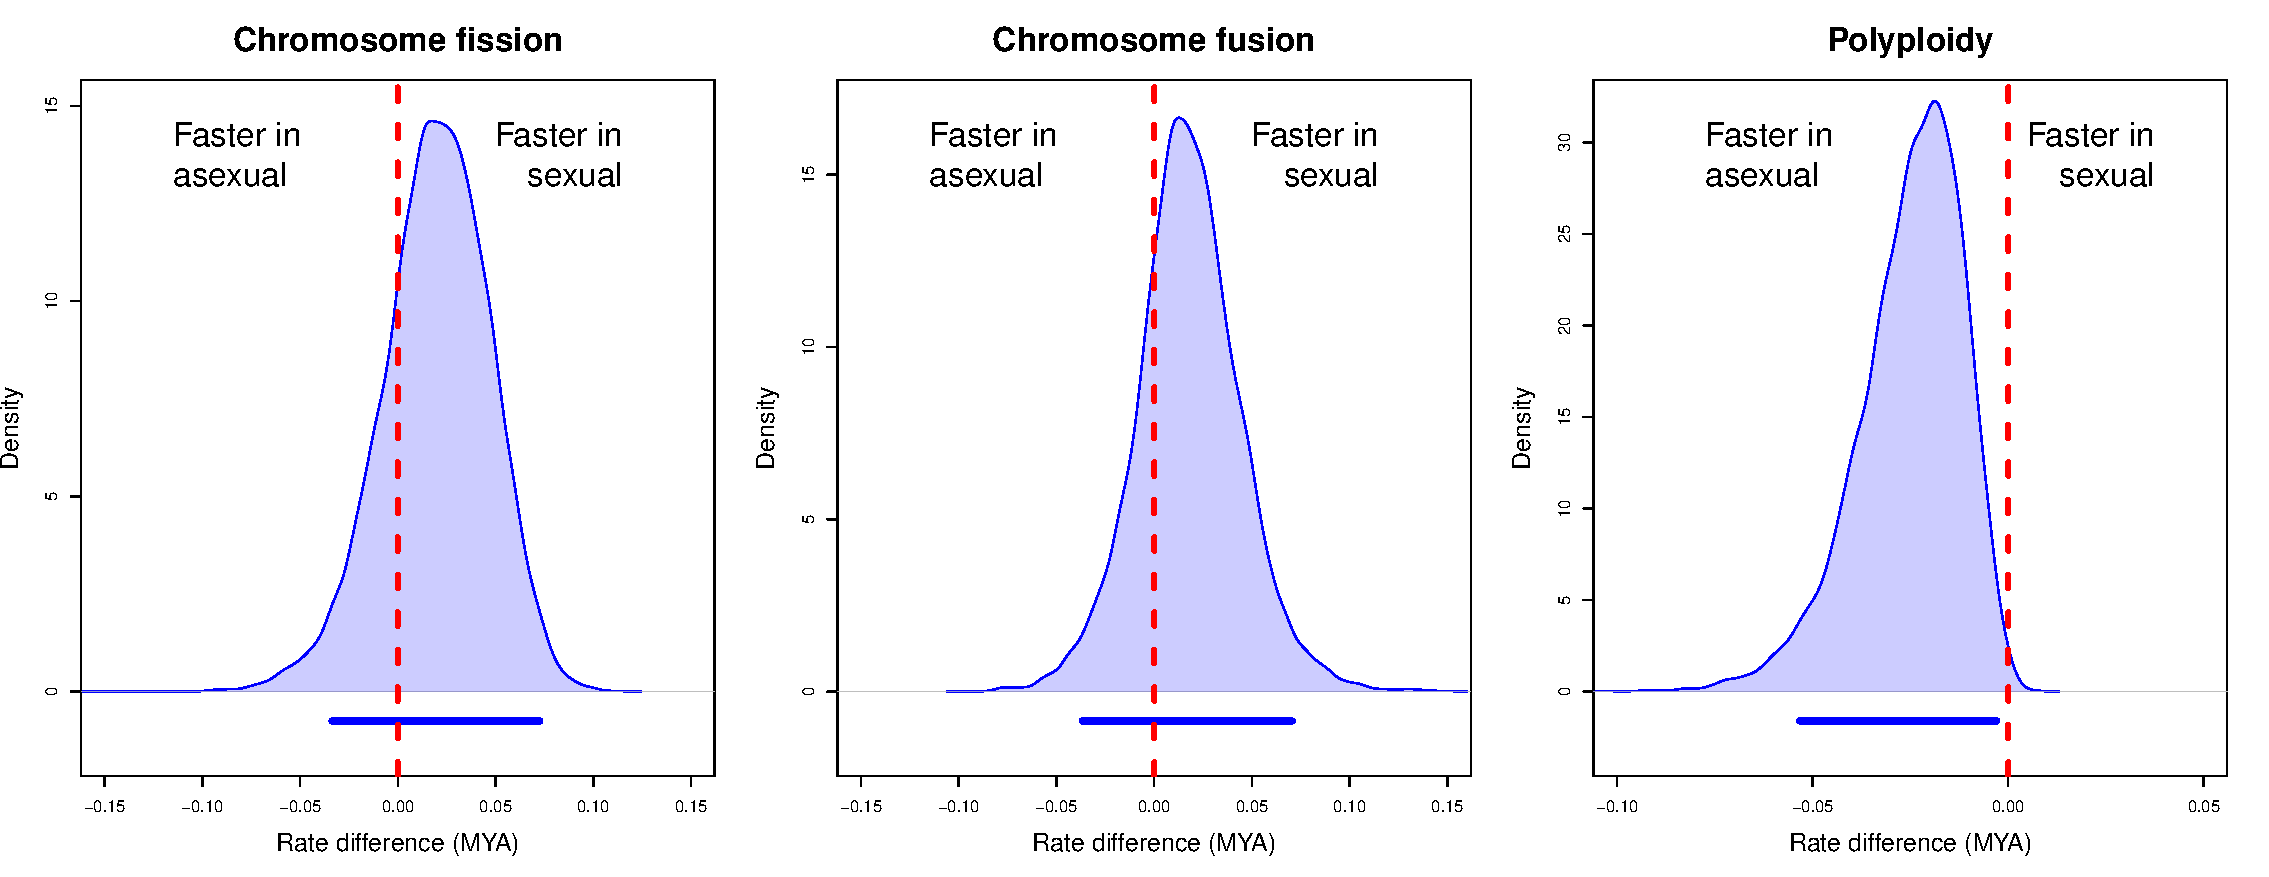
\includegraphics[width=1\textwidth]{figures/phasmatodea_sex_asex_plot.pdf}
\caption{
Rates of chromosome evolution in sexual and asexual lineages in Phasmatodea. 
Bars below the plot indicates the 95\% HPD interval}
\label{fig:phas.plot}
\end{figure}

\begin{figure}
\centering 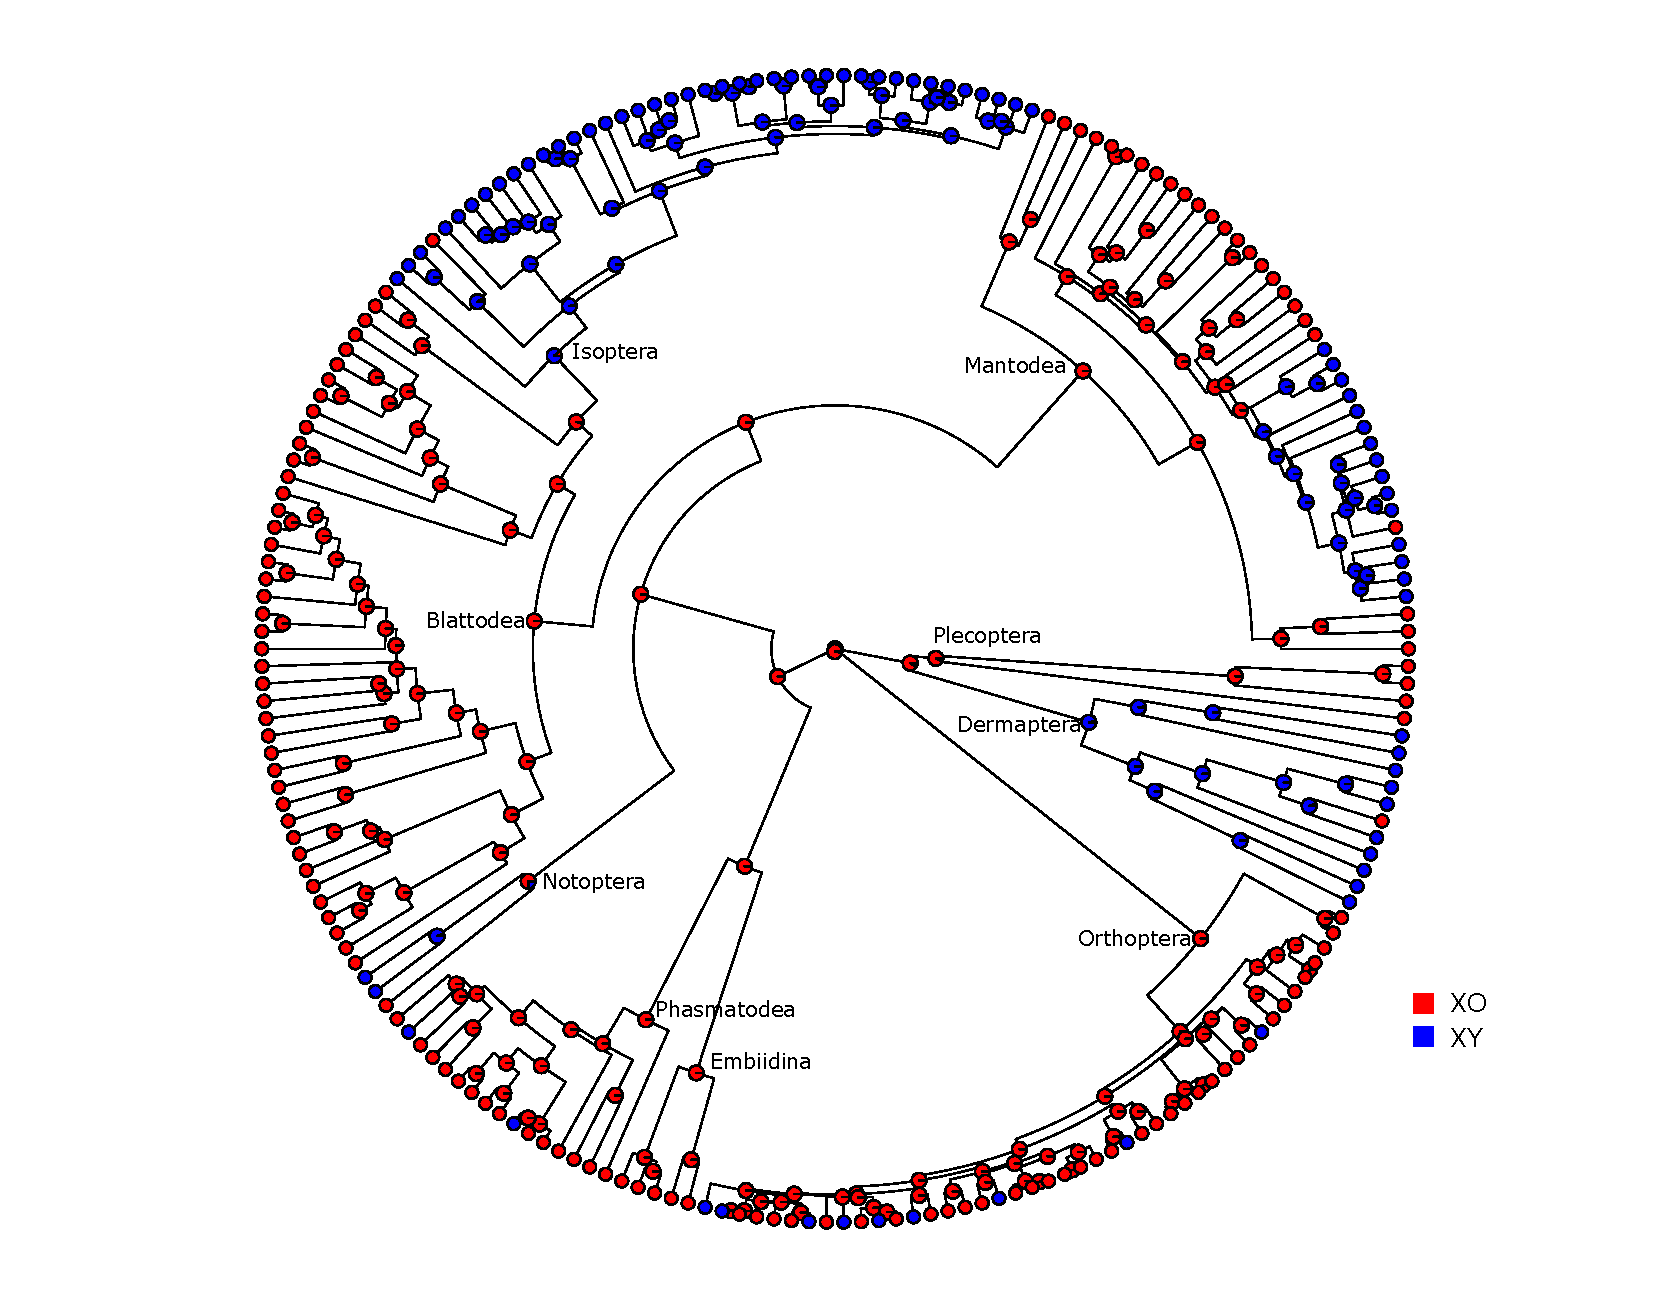
\includegraphics[width=1\textwidth]{figures/sex_chrom_asr_phylogeny.pdf}
\caption{
Ancestral states reconstruction of the sex chromosome systems. This is a single tree of the posterior distribution. Red colour represents the XO sex chromosome system and Blue colour represents the XY sex chromosome system. Order names are marked at the origin of each order. The probabilities of each sex chromosome system as being the ancestral state is given by the respective coloured portion of the pie charts at each node. Tip colours represent the current state of the sex chromosome system.}
\label{fig:sex.asr.plot}
\end{figure}

\begin{figure}
\centering 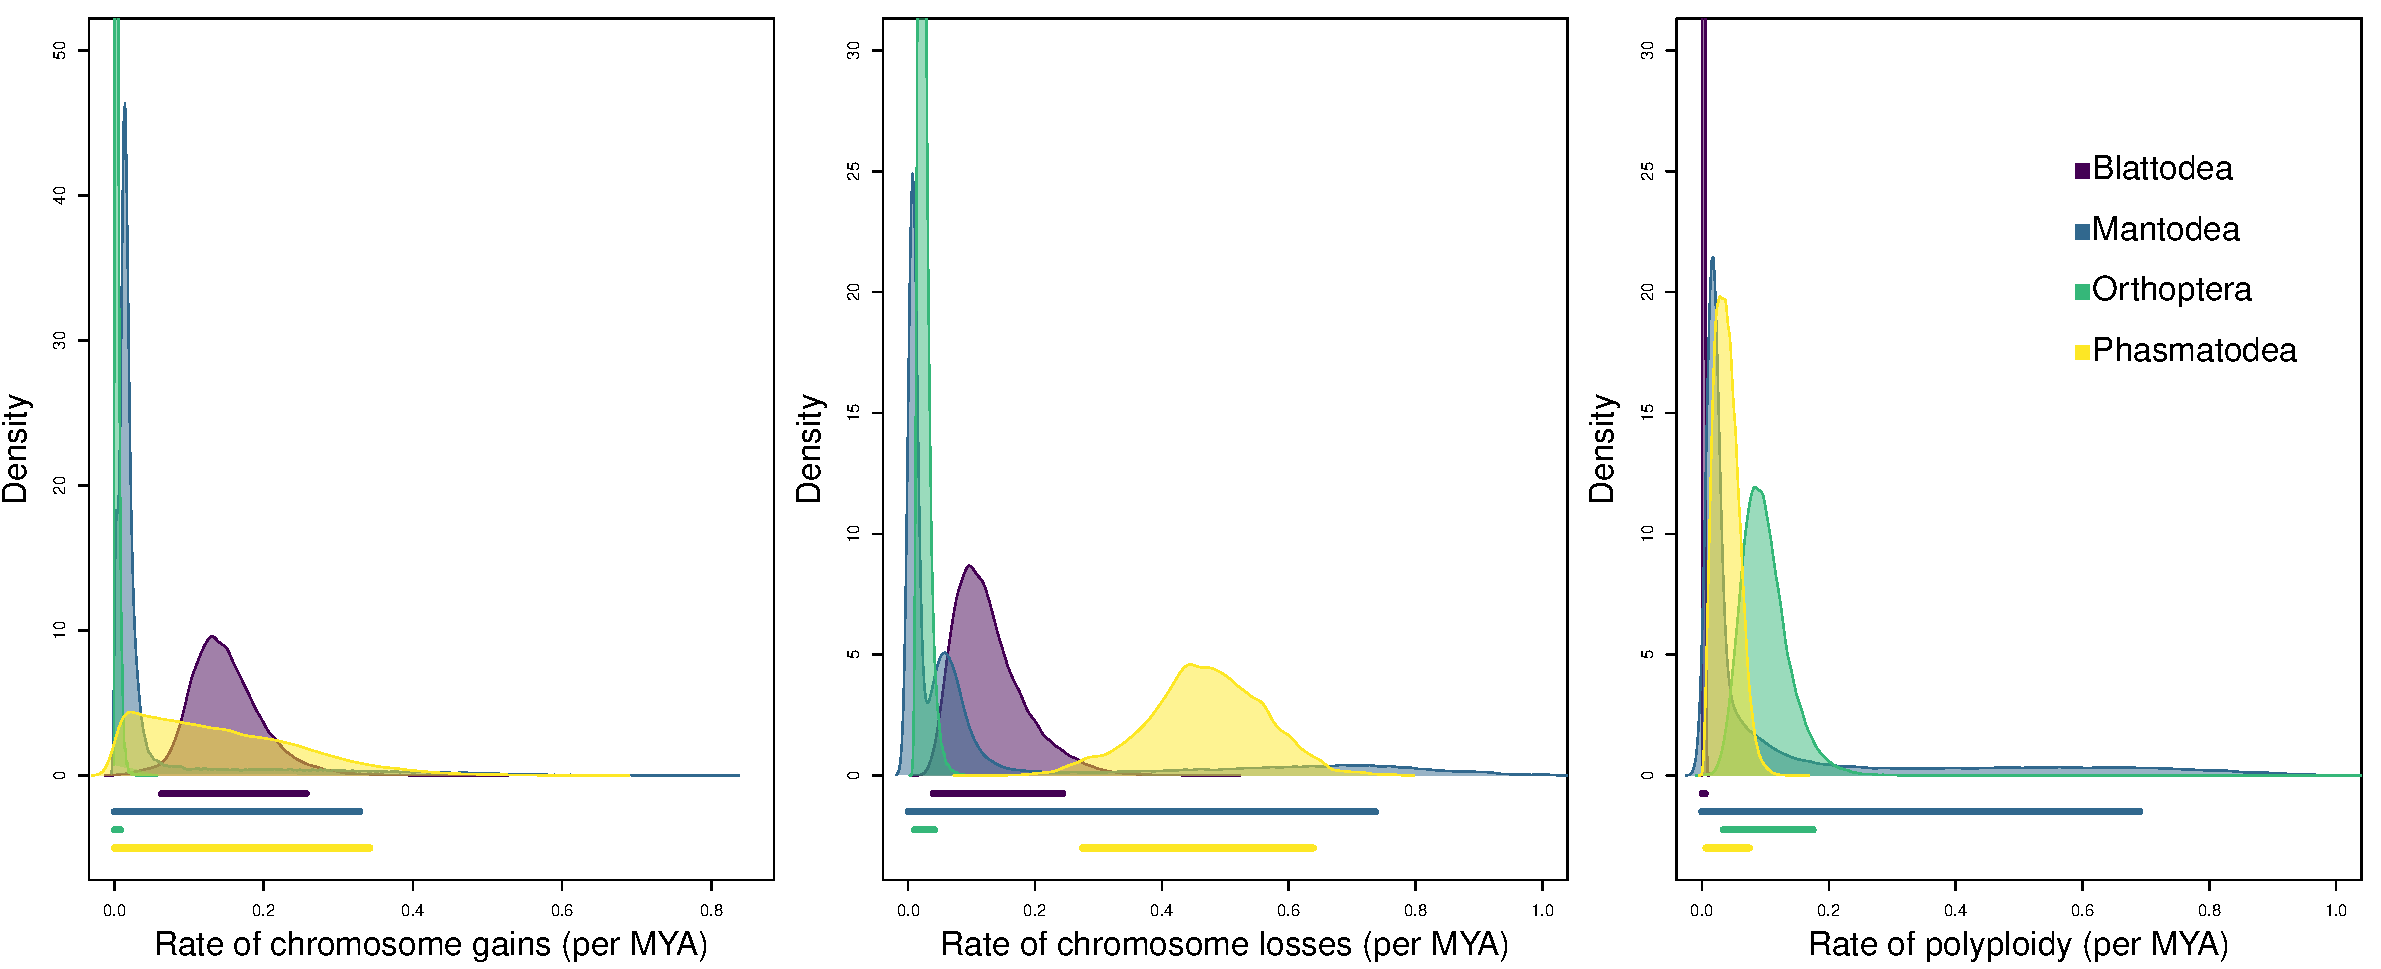
\includegraphics[width=1\textwidth]{figures/order_rates_95HPD.pdf}
\caption{Rates of chromosome fusion, fission, and polyploidy of four orders in the insect clade Phasmatodea. The y-axis is shortened to show the spread of these rates. The bars below each distribution indicates the 95\% HPD interval.}
\label{fig:order.rates.95HPD}
\end{figure}

